%%%%%%%%%%%%%%%%%%%%%%%%%%%%%%%%%%%%%%%%%
% MSc BIS Thesis 
% LaTeX Template
% Version 1.0 (29/08/2014)
%
% Original authors:
% Steven Gunn 
% Sunil Patel
%
% Further authors:
% Michael Stauffer
% 
% This template is based on
% http://www.latextemplates.com/template/masters-doctoral-thesis
%
% License:
% CC BY-NC-SA 3.0 (http://creativecommons.org/licenses/by-nc-sa/3.0/)
%
%%%%%%%%%%%%%%%%%%%%%%%%%%%%%%%%%%%%%%%%%

%----------------------------------------------------------------------------------------
%	PACKAGES AND OTHER DOCUMENT CONFIGURATIONS
%----------------------------------------------------------------------------------------

% For digital publication it is recommended to use a one-sided layout
\documentclass[11pt, oneside]{Thesis}
\addbibresource{Bibliography.bib}

% For printing it is recommended to use a two-sided layout
%\documentclass[11pt, twoside]{Thesis}

\makeglossaries

\begin{document}

%----------------------------------------------------------------------------------------
%	DOCUMENT VARIABLES
%	Fill in the lines below to update the thesis template
%	
%   If you want to cite each of the variables defined below, look at the
%	section above for the citation command.
%----------------------------------------------------------------------------------------

% You thesis title
% Citation command \thesisTitle
\thesisTitle{HAI-BEMS: \\A Hybrid Artificial Intelligent Approach for Building Energy Management Systems}
%-------------------------------------------------  

% You supervisor's name Unicam or FHNW
% Citation command \supName 
\supervisor{Dr. Emanuele \textsc{Laurenzi}}
%-------------------------------------------------  

% You supervisor's URL 
% Citation command \supURL
\supervisorURL{https://www.fhnw.ch/en/people/emanuele-laurenzi}
%-------------------------------------------------

% You supervisor's name Unicam or FHNW
% Citation command \supName 
\supervisorTwo{Prof. Michela \textsc{Quadrini}}

%-------------------------------------------------  

% You supervisor's URL
% Citation command \supURL
\supervisorTwoURL{https://computerscience.unicam.it/michela-quadrini}
%-------------------------------------------------


% If you don't have a co-supervisor, exchange with
\cosupervisorfalse
%\cosupervisortrue
%-------------------------------------------------

% You co-supervisor's name 
% Citation command \supcoName 
%\cosupervisor{Dr. James \textsc{Allan}}
%-------------------------------------------------  

% You co-supervisor's URL
% Citation command \supcoURL
\cosupervisorURL{https://www.empa.ch/web/alja}
%-------------------------------------------------

% Your degree name
% Citation command \degreeName
\degree{Business Information Systems}
\degreeTwo{Computer Science}
%-------------------------------------------------   

% Your name
% Citation command \authorName
\authors{Piermichele \textsc{Rosati}}
\matricola{124176}%
\academicyear{2023/2024}%
%-------------------------------------------------

% Your URL
% Citation command \authorURL
\authorsURL{http://www.johnsmith.com}
%-------------------------------------------------

% Your address (not used)
% Citation command \addressNames
\addresses{}
%-------------------------------------------------

% Your subject area (not used) 
% Citation command \subjectName
\subject{}
%-------------------------------------------------   

% Keywords for your thesis (not used)
% Citation command \keywordNames 
\keywords{}
%-------------------------------------------------

% http://www.fhnw.ch
% Citation command \fhnwURL 
%-------------------------------------------------

% University of Applied Sciences and Arts Northwestern Switzerland
% Citation command \fhnw 
%-------------------------------------------------

% UNIVERSITY OF APPLIED SCIENCES AND ARTS NORTHWESTERN SWITZERLAND
% Citation command \FHNW 
%-------------------------------------------------

% http://www.fhnw.ch/business
% Citation command \hswURL 
%-------------------------------------------------

% School of Business
% Citation command \hsw 
%-------------------------------------------------

% SCHOOL OF BUSINESS
% Citation command \HSW 
%-------------------------------------------------

% http://www.fhnw.ch/business/iwi
% Citation command \iwiURL 
%-------------------------------------------------

% Institute for Information Systems
% Citation command \iwi 
%-------------------------------------------------

% INSTITUTE FOR INFORMATION SYSTEMS for Information Systems
% Citation command \IWI
%-------------------------------------------------

%----------------------------------------------------------------------------------------
%	GLOSSARY
%	Add your glossary terms below
%	
%   If you want to cite a glossary term simply use \gls{term) for the singular form 
%   of the term or \glspl{term} for the plural form of the term.
%----------------------------------------------------------------------------------------

\newglossaryentry{Java}{
    name={Java},
    description={\blindtext}
}

\newglossaryentry{Oracle}{
    name={Oracle},
    description={\blindtext}
}

\newglossaryentry{Microsoft}{
    name={Microsoft},
    description={\blindtext}
}

%----------------------------------------------------------------------------------------
%	ABBREVIATIONS
%	Add your glossary terms below
%	
%   If you want to cite an abbreviation term simply use \gls{term) for the singular form  
%   of the term or \glspl{term} for the plural form of the term.
%----------------------------------------------------------------------------------------

\newacronym{rq}{RQ}{Research Question}
\newacronym{kg}{KG}{Knowledge Graph}
\newacronym{ai}{AI}{Artifical Intelligence}
\newacronym{bems}{BEMS}{Building Energy Management System}
\newacronym{gnn}{GNN}{Graph Neural Network}
\newacronym{ml}{ML}{Machine Learning}
\newacronym{dl}{DL}{Deep Learning}
\newacronym{iot}{IoT}{Internet of Things}
\newacronym{cnn}{CNN}{Convolutional Neural Network}
\newacronym{rnn}{RNN}{Recurrent Neural Network}
\newacronym{dnn}{DNN}{Deep Neural Network}
\newacronym{rdf}{RDF}{Resource Description Framework}
\newacronym{rdfs}{RDFS}{RDF Schema}
\newacronym{uri}{URI}{Uniform Resource Identifier}
\newacronym{owl}{OWL}{Web Ontology Language}
\newacronym{sparql}{SPARQL}{SPARQL Protocol and RDF Query Language}
\newacronym{nlp}{NLP}{Natural Language Processing}
\newacronym{lod}{LOD}{Linked Open Data}
\newacronym{kge}{KGE}{Knowledge Graph Embedding}
\newacronym{gcn}{GCN}{Graph Convolutional Network}
\newacronym{gat}{GAT}{Graph Attention Network}
\newacronym{mpnn}{MPNN}{Message Passing Neural Network}
\newacronym{graphsage}{GraphSAGE}{Graph Sample and Aggregation}

% PDF meta-data
\hypersetup{pdftitle={\thesisTitle}}
\hypersetup{pdfsubject=\subjectName}
\hypersetup{pdfauthor=\authorName}
\hypersetup{pdfkeywords=\keywordNames}

\frontmatter % Use roman page numbering style (i, ii, iii, iv...) for the pre-content pages

%----------------------------------------------------------------------------------------
%	TITLE PAGE
%----------------------------------------------------------------------------------------

\titlePage

%----------------------------------------------------------------------------------------
%	ABSTRACT PAGE
%----------------------------------------------------------------------------------------

\abstract{
    The Thesis Abstract is written here (and usually kept to just this page)\ldots
}

\clearpage % Start a new page

%----------------------------------------------------------------------------------------
%	STATEMENT OF AUTHENTICITY
%----------------------------------------------------------------------------------------

\fillingPage{} 
\statementOfAuthenticity

\clearpage

%----------------------------------------------------------------------------------------
%	TABLE OF CONTENTS
%----------------------------------------------------------------------------------------

\tableofcontents

%----------------------------------------------------------------------------------------
%	THESIS CONTENT - CHAPTERS
%----------------------------------------------------------------------------------------

\mainmatter % Begin numeric (1,2,3...) page numbering

\fillingPage{}
\chapter{Introduction}\label{chap:intro}
The remainder of the paper is structured as follows:
\section{Background}\label{sec:background}

\section{Problem Statement}\label{sec:problem-statement}

\section{Thesis Statement}\label{sec:thesis-statement}

\section{Research Questions}\label{sec:research-questions}
The main \gls{rq}:

How can a Graph Neural Network (GNN) support IoT data classification in KGs about BEMS? 
\fillingPage{}
\chapter{Literature Review}\label{chap:literature-review}

\section{Knowledge Graphs}\label{sec:knowledge-graphs}
\glspl{kg} have came up as a key technology in the field of data management and \gls{ai}, enabling sophisticated data integration, retrieval and analysis, and analysis.
This section provides an in-depth examination of \glspl{kg}, their theoretical foundations, practical applications and recent advances.

\subsection*{Theoretical Foundations of Knowledge Graphs}
\subsubsection*{Definition and Structure}
\glspl{kg} are directed graph-based data structures that represent real-world entities and their interrelations, providing a way to model complex domains and their underlying semantics.
A \gls{kg} consists of nodes (also called entities) and edges (also called relationships), forming a network of interconnected information.
This structure allows \glspl{kg} to capture rich contextual information and provide a semantic framework for data (\cite{Hogan2021}).
In other words, a \gls{kg} refers to a semantic network graph which is consisted of diverse entities, concepts, and relationships.
It is used to formally describe various things and their associations in the real world.
\glspl{kg} are generally represented in triples $\gls{kg}=\{\mathnormal{E,R,F}\}$.
\begin{itemize}
    \item $E$ represents the entity set $\{\mathnormal{e_1, e_2, ... ,e_E} \}$, and the entity $e$ is the most basic element in the \gls{kg}, referring to the items that exist objectively and can be distinguished from each other.
    \item $R$ represents the relation set $\{\mathnormal{r_1, r_2, ... ,r_R}\}$, and the relation $r$ is an edge in the \gls{kg}, representing a specific connection between different entities.
    \item $F$ represents the fact set $\{\mathnormal{f_1,f_2, ... ,f_F}\}$, and each $\mathnormal{f}$ is defined as a triple $(\mathnormal{h,r,t}) \in \mathnormal{f}$, in which $\mathnormal{h}$ denotes the head entity, $\mathnormal{r}$ stands for the relationship, and $\mathnormal{t}$ indicates the tail entity.
\end{itemize}

The \gls{kg} in Fig. \ref{fig:kg-example-albert-einstein} visually represents some relationships and attributes associated with Albert Einstein.
At the center of the graph is ``Albert Einstein'', from which several connections extend.
One connection indicates that he was ``born in'' Germany.
Another connection shows his ``occupation'' as a ``Theoretical Physicist''.
This occupation is further connected to ``Physicist'' as a ``kind of'' category, indicating that a theoretical physicist is a type of physicist.
The graph also shows that a physicist ``practices'' physics.
Additionally, it highlights that Albert Einstein ``developed'' the ``Theory of Relativity'', which is shown as a ``branch of'' physics.
The graph effectively maps out key aspects of Albert Einstein's background, profession, and contributions to science.

\begin{figure}[htbp]
    \centering
 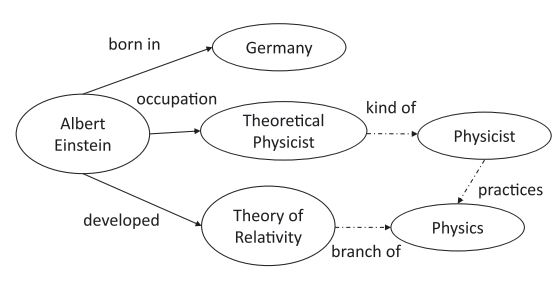
\includegraphics[width=.7\textwidth]{03_Figures/literature-review/kg-example-albert-einstein.png}
     \rule{35em}{0.5pt}
    \caption{An example of \acrlong{kg} (\cite{Chaudhri2022})} 
 \label{fig:kg-example-albert-einstein}
\end{figure}

\subsubsection*{Ontologies and Semantic Web Technologies}
An ontology is a formal representation of knowledge in a domain, specifying the concepts, relationships, and constraints that exist within that domain. The term ``ontology'' can be used to the shared understanding of some domain of interest (\cite{Uschold1996}).
Ontologies play a critical role in defining the schema and semantics of \glspl{kg}. They specify the types of entities, relationships, and constraints, thereby providing a formalized structure for the data. The Semantic Web technologies, particularly the \gls{rdf} and the \gls{owl}, are fundamental to the development and functioning of \glspl{kg} (\cite{Antoniou2008}).
\\\gls{rdf} is a standard model for data interchange on the web.
\gls{rdf} is a part of the \gls{w3c}'s Semantic Web activity and provides a model for data interchange on the Web.
It uses triples $\langle subject,predicate,object \rangle$ to represent information, providing a flexible and extensible framework for creating and managing \glspl{kg} (\cite{Cyganiak14RCA}).
The subject is the resource being described, the predicate is the property or characteristic of the subject, and the object is the value of the property, that can be literals, which are concrete data values such as strings, numbers, or dates..
\gls{rdf} uses \glspl{uri} to uniquely identify subjects and predicates, ensuring that resources are globally identifiable.
\gls{rdf} can be serialized in various syntaxes, including \gls{rdf}/XML, Turtle, N-Triples, and JSON-LD. \gls{rdf}/XML is the original \gls{rdf} syntax using XML to represent \gls{rdf} triples. Turtle is a more human-readable syntax for \gls{rdf} data, concise and easier to write and read compared to \gls{rdf}/XML. N-Triples is a plain text format for encoding \gls{rdf} triples, useful for streaming data or simple data exchange. JSON-LD is a JSON-based format to serialize Linked Data, designed to be easy to use and integrate with existing JSON-based systems.
\gls{rdfs} is a semantic extension of \gls{rdf} that provides mechanisms to describe groups of related resources and the relationships between these resources. It allows for defining classes, which are categories of resources; properties, which are relationships between resources; and hierarchies, enabling inheritance.
\gls{rdf} is widely used in various domains, including the Semantic Web, where it enables the creation of a web of data with meaning, allowing machines to understand and process web content; \glspl{kg}, powering large-scale graph-based data structures used by organizations like Google and Amazon (\cite{Kejriwal2022}); data integration, integrating data from disparate sources by providing a common data model; and ontology engineering, defining and using ontologies to model domain knowledge. \gls{rdf} provides a robust and flexible framework for representing structured information, enabling interoperability and integration of data across different systems and domains.
\\\gls{owl} is used to explicitly represent the meaning of terms in vocabularies and the relationships between those terms. It enables more complex and expressive representations compared to \gls{rdfs} (\cite{Deborah2004}).
The \gls{owl} standard is a \gls{w3c} technology for defining and using web ontologies, enhancing \gls{rdf} by offering greater expressiveness for complex information. \gls{owl} ontologies consist of classes, properties, and individuals, enabling detailed descriptions of relationships and characteristics. It supports complex class expressions, including logical operators and restrictions like cardinality and property constraints.
\gls{owl} has three sublanguages: \gls{owl} Lite (simple feature set), \gls{owl} DL (maximum expressiveness with computational guarantees), and \gls{owl} Full (greatest expressiveness without computational guarantees). Reasoning capabilities in \gls{owl} allow for inferring implicit knowledge, consistency checking, and classification.
\gls{owl} is used in knowledge management, information integration, and semantic search, providing a common framework for understanding and integrating data. It promotes interoperability and the creation of semantically rich, interconnected web data.

\subsubsection*{Query Languages}
\gls{sparql} is the standard query language for retrieving and manipulating data stored in \gls{rdf} format. It allows users to write complex queries to extract specific information from a \gls{kg}, making it a powerful tool for data analysis and knowledge discovery (\cite{Jorge2009}).
It allows users to query \gls{rdf} data by specifying patterns of triples and to update \gls{rdf} data by inserting, deleting, and modifying \gls{rdf} triples. \gls{rdf} is a foundation for Linked Data, which involves interlinking data across the web using \glspl{uri} and \gls{rdf}. This enables the creation of a web of data that can be easily connected and queried.

Cypher is another query language for graph databases, such as Neo4j, that allows users to interact with graph data using a pattern-matching syntax. Cypher queries are used to traverse the graph, retrieve specific patterns, and perform operations on the data (\cite{Francis2018}).
Cypher supports complex queries involving multiple nodes and relationships, aggregation, sorting, and limiting results. It also provides functions for working with strings, numbers, dates, and collections, as well as support for subqueries and variable-length paths.
Cypher is widely used for graph analytics, network analysis, and data exploration, enabling users to easily express complex graph traversals and operations. It leverages Neo4j's indexing and optimization capabilities to ensure efficient execution of queries, making it a powerful tool for working with connected data.

\subsection*{Applications of Knowledge Graphs}

\subsubsection*{General Applications}
\glspl{kg} have been adopted across various domains due to their ability to integrate heterogeneous data sources, provide semantic context, and enable advanced querying and reasoning.
According to \cite{Kapanipathi2020}, in healthcare \glspl{kg} are used to integrate patient records, clinical trials, research data, and medical ontologies, enabling personalized medicine and decision support systems. They help in identifying relationships between diseases, treatments, and patient outcomes.
\\Financial institutions leverage \glspl{kg} to connect data from various sources, such as market data, regulatory information, and customer transactions. This integration facilitates risk management, fraud detection, and compliance monitoring (\cite{Tchechmedjiev2019}).
\\In e-commerce, \glspl{kg} enhance product recommendation systems by linking customer preferences, purchase history, and product information. They enable more personalized and relevant recommendations, improving customer satisfaction and sales (\cite{Zhang2021}).

In compliance with \cite{Zou2020}, Fig. \ref{fig:kg-application-fields} shows a mind map illustrating the main applications of knowledge graphs. It divides the applications into five main categories: question answering, recommendation systems, information retrieval, domain-specific applications and other applications. With regard to question answering, methods based on semantic parsing, methods based on information retrieval, methods based on embedding, methods based on \gls{dl} and more complex tasks are included.
\glspl{kg} significantly enhance search engines by providing semantic search capabilities. They enable the understanding of user queries in context, allowing for more accurate and relevant search results. Google's Knowledge Graph is a prominent example, enhancing search results with information about entities and their relationships (\cite{singhal2012introducing}).
Recommender systems are classified into embedding-based methods, path-based methods and other methods. Information retrieval includes query representation, document representation, ranking and \gls{dl}. Domain-specific applications include medicine, computer security, finance, news and education.
Within enterprises, \glspl{kg} are used to manage and utilize internal knowledge effectively. They integrate data from different departments, such as human resources, finance, and operations, providing a unified view of the organization's information. This integration supports decision-making, collaboration, and innovation (\cite{pujara2013knowledge}).
Other applications include social networks, classification, geosciences and various other applications.

\begin{figure}[htbp]
	   \centering
    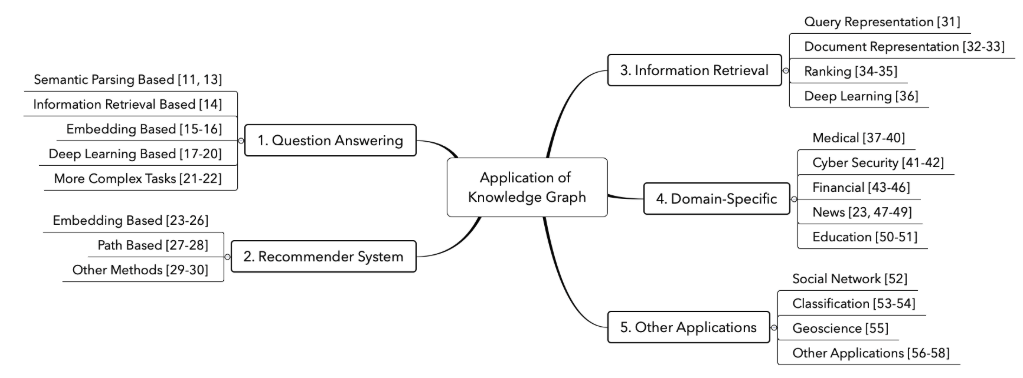
\includegraphics[width=\textwidth]{03_Figures/literature-review/kg-application-fields.png}
		\rule{35em}{0.5pt}
	   \caption{Application of \acrlongpl{kg} (\cite{Zou2020})} 
    \label{fig:kg-application-fields}
\end{figure}

\subsection*{Recent Advancements in Knowledge Graphs}

\subsubsection*{Integration with Machine Learning}
Recent research has focused on integrating \glspl{kg} with \gls{ml} and \gls{dl} techniques to enhance their capabilities and applications. These integrations have led to significant advancements in various areas, including \gls{nlp}, recommendation systems, and predictive analytics.
\begin{itemize}
    \item \textbf{\glspl{kge}}: \gls{kge} techniques represent entities and relationships in a continuous vector space, enabling the use of \gls{ml} algorithms for tasks such as link prediction, entity classification, and clustering. Popular methods include TransE (\cite{Bordes2013}), TransH (\cite{Wang2014}), and TransR (\cite{Lin2015}), each providing different ways to model relationships in the embedding space (\cite{Wang2017}).
    \item \textbf{\glspl{gnn}}: \glspl{gnn} are \gls{dl} models designed to operate on graph-structured data. They leverage the relational nature of graphs to perform tasks such as node classification, link prediction, and graph classification. \glspl{gnn} have been successfully applied to enhance the capabilities of \glspl{kg} in various domains (\cite{Wu2021}).
    
    Section \ref{sec:graph-neural-networks} provides a comprehensive and in-depth description of \glspl{gnn}.
\end{itemize}

\subsubsection*{Natural Language Processing and Question Answering}
\glspl{kg} have been instrumental in advancing \gls{nlp} applications, particularly in question answering systems. By providing structured and semantically rich information, \glspl{kg} enable systems to understand and generate human language more effectively.
\glspl{kg} support question answering systems by enabling them to retrieve and reason over structured data.
These systems can answer complex queries by traversing the graph and applying logical inferences based on the relationships between entities (\cite{Yasunaga2021}).
\glspl{kg} enhance text analysis and semantic search by providing contextual information about entities mentioned in the text.
This contextual understanding improves the accuracy of information retrieval and the relevance of search results (\cite{Fernandez2011}).

\subsection*{Challenges and Future Directions}

\subsubsection*{Scalability and Performance}
As \glspl{kg} grow in size and complexity, scalability and performance become critical challenges. Efficient storage, querying, and updating of large \glspl{kg} require advanced techniques and architectures. Research in distributed computing, graph databases, and parallel processing is ongoing to address these issues (\cite{Chaudhri2022}).
 
\subsubsection*{Data Quality and Integration}

Ensuring the accuracy and consistency of data in \glspl{kg} is essential for their reliability. Data quality issues, such as inconsistencies, duplications, and inaccuracies, can significantly impact the performance of applications relying on \glspl{kg}. Developing methods for automatic data cleaning, validation, and integration is an active area of research (\cite{Paulheim2017}).

\subsubsection*{Privacy and Security}

The integration of sensitive data into \glspl{kg} raises concerns about privacy and security. Protecting personal and confidential information while allowing for meaningful data analysis is a significant challenge. Research is focusing on developing techniques for secure data sharing, access control, and anonymization within \glspl{kg} (\cite{Bonatti2017}).

\subsubsection*{Interoperability and Standardization}

Interoperability and standardization are crucial for the widespread adoption of \glspl{kg}. Ensuring that different \glspl{kg} can work together seamlessly and that their data can be easily integrated requires the development of common standards and protocols. Efforts such as the \gls{lod} initiative and \gls{w3c} standards aim to address these challenges (\cite{Bizer2023}).

\subsection*{Conclusion}
\glspl{kg} represent a transformative technology for data integration, retrieval, and analysis, offering significant benefits across various domains. Their ability to provide semantic context and capture complex relationships makes them invaluable for applications in healthcare, finance, e-commerce, and enterprise knowledge management. Recent advancements in \gls{ml}, particularly in the integration with \glspl{gnn}, have further enhanced the capabilities of \glspl{kg}, opening new avenues for research and application. However, challenges related to scalability, data quality, privacy, and interoperability remain and must be addressed to fully realize the potential of \glspl{kg}. Continued research and development in these areas will be crucial for the future evolution and adoption of \glspl{kg}.

\section{Graph Neural Networks}\label{sec:graph-neural-networks}

\section{Building Energy Management Systems}\label{sec:building-energy-management-systems}


\fillingPage{}
%\chapter{Research Method}\label{chap:research-method}
\fillingPage{} 
\chapter{Conclusion}\label{chap:conclusion}

%----------------------------------------------------------------------------------------
%	BIBLIOGRAPHY
%----------------------------------------------------------------------------------------

\fillingPage{}
\nocite{*}
\listOfBibliography

%----------------------------------------------------------------------------------------
%	GLOSSARY (if appropriate)
%----------------------------------------------------------------------------------------

% \fillingPage{}
% \listOfGlossary

%----------------------------------------------------------------------------------------
%	ABBREVIATIONS (if appropriate)
%----------------------------------------------------------------------------------------
\fillingPage{}
\listOfAbbreviation

%%----------------------------------------------------------------------------------------
%%	LIST OF FIGURES (optional)
%%----------------------------------------------------------------------------------------

\fillingPage{} 
\listOfFigures

%%----------------------------------------------------------------------------------------
%%	LIST OF TABLES (optional)
%%----------------------------------------------------------------------------------------

\fillingPage{} 
\listOfTables

%----------------------------------------------------------------------------------------
%	THESIS CONTENT - APPENDICES (if appropriate)
%----------------------------------------------------------------------------------------

\appendix % Cue to tell LaTeX that the following 'chapters' are Appendices

% Include the appendices of the thesis as separate files from the Appendices folder
% Uncomment the lines as you write the Appendices

% \fillingPage{} 
% % Appendix A

\chapter{Appendix Title Here} % Main appendix title

\label{AppendixA} % For referencing this appendix elsewhere, use \ref{AppendixA}

\addtocontents{toc}{\vspace{1em}} % Add a gap in the Contents, for aesthetics

Write your Appendix content here.

% \fillingPage{} 
% % Appendix A

\chapter{Appendix Title Here} % Main appendix title

\label{AppendixB} % For referencing this appendix elsewhere, use \ref{AppendixA}

\addtocontents{toc}{\vspace{1em}} % Add a gap in the Contents, for aesthetics

Write your Appendix content here.

%\fillingPage{} 
%\input{02_Appendices/AppendixC}

%----------------------------------------------------------------------------------------
%	FOREWORD / ACKNOWLEDGEMENTS (optional)
%----------------------------------------------------------------------------------------

\ackPage{
    The acknowledgements and the people to thank go here, don't forget to include your project advisor\ldots
}

\clearpage % Start a new page

\backmatter

\end{document}  